\documentclass[a4paper, 11pt]{article}

\usepackage{amsmath, amssymb, amstext, amsfonts, mathrsfs}	% Mathe
\usepackage[applemac]{inputenc}	% Direkte Eingabe von Umlauten und anderen Diakritika
\usepackage{hyperref}		%Anklicken von Links
\usepackage[normalem]{ulem}	%weitere Formatierung von Schriften
\usepackage{fancyhdr}		%sch\"one Kopf- und Fußzeilen
\usepackage[ngerman]{babel}	%deutsche Sprache
\usepackage{verbatim}
\usepackage{graphicx}

\pagestyle{fancy}
\lhead{SEIII: Logikprogrammierung\\}
\chead{\ \\(L. Kruse: 6659482, A. Hildebrandt: 6688865, E. Baalmann: 6704003)}
\rhead{\today\\}

\parindent0pt

\begin{document}
\setcounter{section}{5}
\section{Rekursive Berechnungen/rekursive Strukturen}
\subsection{Numerische Rekursion}
\subsection*{1.1}

Rekursiver Aufstieg:

\begin{verbatim}
%goldener_schnitt(+Schritte, ?Resultat)
 goldener_schnitt(0, 2).
 goldener_schnitt(Schritte, Resultat) :- 
   Schritte > 0, Schritte2 is Schritte - 1,
   goldener_schnitt(Schritte2, Resultat2), Resultat is 1 / Resultat2 + 1.
\end{verbatim}

Rekursiver Abstieg (mit Endrekursion):

\begin{verbatim}
%goldener_SchnittE(+Schritte, +Akk, ?Res)
 goldener_SchnittE(0,Akk,Res) :- Res = Akk.
 goldener_SchnittE(Schritte, Akk, Res) :- 
   Schritte > 0, Schritte1 is Schritte - 1, Akk1 is 1 / Akk + 1, 
   goldenerSchnittE(Schritte1, Akk1, Res).
\end{verbatim}

\subsection*{1.2}

\begin{verbatim}
time(goldener_schnitt(1000000, Res)).
% 2,999,998 inferences, 93.641 CPU in 94.010 seconds

time(goldenerSchnittE(1000000, 1, Res)).
% 3,000,001 inferences, 0.344 CPU in 0.340 seconds
\end{verbatim}

Wie am Rechenzeitbedarf zu sehen ist, arbeitet der Rekursive Abstieg drastisch schneller als der Rekursive Aufstieg. Die Verst\"andlichkeit des Pr\"adikates verringert sich dabei nur gering, da man lediglich einen Akkumulator einbauen musste.

\subsection*{1.3}

Das Pr\"adikat ist ineffizient, weil es zwei rekursive Aufrufe ben\"otigt. Wenn man sich bei der Rekursion auf einen Aufruf beschr\"ankt, l\"asst sich die Effizienz stark erh\"ohen.

\begin{verbatim}
%fibonacci(+Schritte, ?Resultat)
 fibonacci(Schritte, Resultat) :- fibonacci_(Schritte, 1, 0, Resultat).
 fibonacci_(0, _, Prev, Prev).
 fibonacci_(1, Val, _, Val).
 fibonacci_(Schritte, Val, Prev, Resultat) :- 
   Schritte >= 0, Schritte2 is Schritte - 1, ValPrev is Val + Prev, 
   fibonacci_(Schritte2, ValPrev, Val, Resultat).
\end{verbatim}

\subsection*{1.4}

\begin{verbatim}
%goldener_schnitt_fib(+Schritte, ?Resultat)
 goldener_schnitt_fib(Schritte, Resultat) :-
   fibonacci(Schritte, Resultat1), Schritte2 is Schritte -1,
   fibonacci(Schritte2, Resultat2), Resultat is Resultat1 / Resultat2.


time(goldener_schnitt_fib(1500, Res)).
% 8,868 inferences, 0.000 CPU in 0.000 seconds
% evaluation error: 'float_overflow'
\end{verbatim}

Ab einer Schrittzahl von ca. 1500 kann Prolog die ben\"otigten Fibonacci Zahlen nicht mehr berechnen. Da die CPU Zeit bei dieser Schrittzahl noch 0 betr\"agt, lassen sich die tats\"achlichen Zeiten nicht mit den Zeiten der naiven L\"osungen vergleichen. Allerdings kann man bei einem Overflow auf so kleiner Schrittzahl annehmen, dass die L\"osung durch Fibonacci sehr ineffizient ist. 

\subsection{Stromorientierte Verarbeitung}

\subsection*{2.1}

\begin{verbatim}
%goldener_schnitt_incr(+Schritte, ?Resultat)
 goldener_schnitt_incr(Schritte, Resultat) :-
   goldener_schnitt_incr_schritt(1, Schritte, Resultat).
    
 goldener_schnitt_incr_schritt(Akku, 0, Akku).
 goldener_schnitt_incr_schritt(Akku, SchrittLinks, Resultat) :-
   SchrittLinks > 0,
   (Resultat is Akku; (
        Zwischen is ((1 / Akku) + 1), SchrittLinksJetzt is SchrittLinks - 1,
        goldener_schnitt_incr_schritt(Zwischen, SchrittLinksJetzt, Resultat))).
\end{verbatim}

\newpage

\subsection*{2.2}

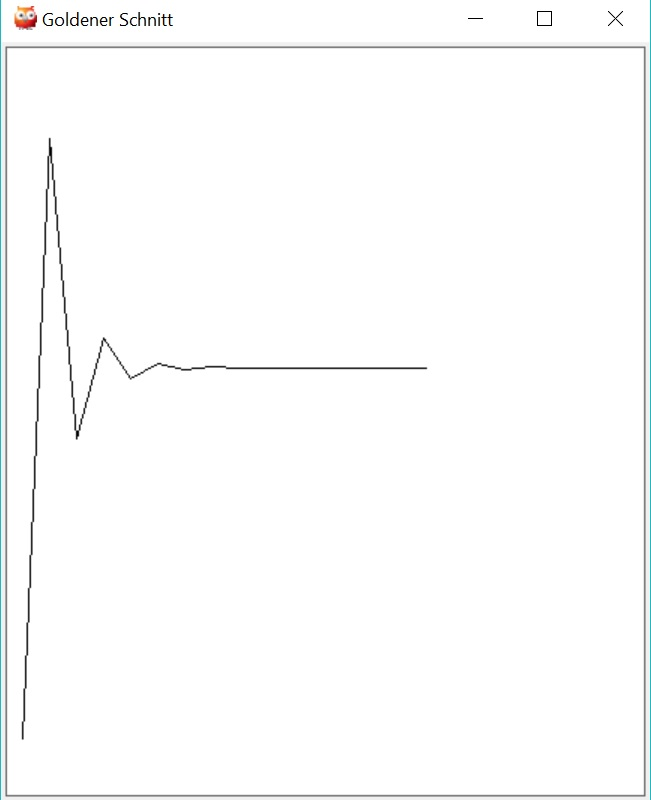
\includegraphics{display.png}\\

Ab neun Approximationsschritten sinkt der Approximationsfehler unter die Darstellungsgenauigkeit.

\subsection{Verzweigende rekursive Strukturen}

\subsection*{3.1}

\begin{verbatim}
%Typtest
baum(A):- atom(A).
baum(s(A,B)):- baum(A),baum(B).
\end{verbatim}

\subsection*{3.2}

\begin{verbatim}
%depth(+Baum, ?Depth)
 depth(Atom,1) :- atom(Atom).
 depth(s(LinkerTeilBaum,_),Depth) :-
   depth(LinkerTeilBaum,Depth2), Depth is Depth2 + 1.
 depth(s(_,RechterTeilBaum),Depth) :-
   depth(RechterTeilBaum,Depth2), Depth is Depth2 + 1.

%depth2(+Baum, ?Depth)
 depth2(Baum,Depth) :- depthENDREK(Baum,0,Depth).
 depthENDREK(Atom,AKK,Depth) :-
   atom(Atom),Depth is AKK + 1.
 depthENDREK(s(LinkerTeilBaum,_),AKK,Depth):-
   AKK2 is AKK + 1, depthENDREK(LinkerTeilBaum,AKK2,Depth).
 depthENDREK(s(_,RechterTeilBaum),AKK,Depth):-
   AKK2 is AKK + 1, depthENDREK(RechterTeilBaum,AKK2,Depth).
\end{verbatim}

\subsection*{3.3}

\begin{verbatim}
%maxDepth(+Baum,?Depth)
 maxDepth(Baum,Depth) :- 
   findall(LocalDepth, depth2(Baum,LocalDepth), L), max_list(L,Depth).
\end{verbatim}

\subsection*{3.4}

\begin{verbatim}
%maxDepthRek(+Baum,?Depth)
 maxDepthRek(Atom, 1) :- atom(Atom).
 maxDepthRek(s(LinkerTeilBaum,RechterTeilBaum),Depth) :-
   maxDepthRek(LinkerTeilBaum,DepthLinks),
   maxDepthRek(RechterTeilBaum,DepthRechts),
   Depth is max(DepthLinks,DepthRechts) + 1.
\end{verbatim}

Die nicht-endrekursive Version ist (wie in den meisten F\"allen) die intuitivere Variante.

\subsection*{3.5}

\begin{verbatim}
%minDepth(+Baum, ?Depth)
 minDepth(Baum,Depth):-
   findall(LocalDepth, depth2(Baum,LocalDepth), L), min_list(L,Depth).
   
%isBalenced(+Baum)
 isBalenced(Baum):-
   minDepth(Baum,MinDepth), maxDepth(Baum,MaxDepth),
   MinDepth + 1 >= MaxDepth.
\end{verbatim}

\end{document}